\documentclass[uplatex,dvipdfmx]{jsarticle}

\usepackage[uplatex,deluxe]{otf} % UTF
\usepackage[noalphabet]{pxchfon} % must be after otf package
\usepackage{stix2} % 欧文&数式フォント
\usepackage[fleqn,tbtags]{mathtools} % 数式関連 (w/ amsmath)
\usepackage{hira-stix} % ヒラギノフォント&STIX2 フォント代替定義(Warning回避)
\usepackage{amsmath}
\usepackage{url}
\usepackage{float} % プリアンブルに追加

\setcounter{tocdepth}{3}
% nothing to insert here
\usepackage{moreverb}
\usepackage{lscape}
%\pagestyle{empty}
%\usepackage{wrapfig}
%\usepackage{url}
%\usepackage{EasyLayout}

\usepackage{ascmac}
\usepackage{xurl}

\begin{document}

\title{危険交差点警告システム}
\author{25G1051 近藤巧望}
%\date{6月12日(木)}
\maketitle
\section{はじめに}
%はじめにのセクションでは,研究の背景や目的を簡潔に記述する.

\subsection{社会的背景}
自転車は温室効果ガスを排出しない移動手段であり,環境に優しい交通手段として注目されている.
また,日本の自転車保有台数は約6870万台(つまり約二人に1台)となっており,自転車は現在でも使う人が多い他,
交通渋滞の緩和や健康促進,地球温暖化等の環境問題への配慮の観点から,政府からも自転車活用推進法に基づき自転車の利用が推奨されている
\cite{ref:koutuusyou_1,ref:koutuusyou_2}.

しかし交通事故に焦点を当てると,自転車搭乗中の事故として出会い頭衝突が原因の事故は
2023年時点では自転車搭乗中事故全体の52.9\%を占めており,高い割合を示している\cite{ref:sonpo_1}.

\subsection{問題点}
\indent
問題点としては,自転車での出会い頭衝突の事故の多さが挙げられる.
出会い頭衝突による事故は,前述の通り自転車搭乗中事故全体の52.9\%を占めている.
また,自転車事故は特に交差点で発生することが多く,これらの場所では視界が遮られたり信号の認識が難しかったりするため,事故が起こりやすい.
さらに,自転車事故の多くは法令違反や不注意によるものであり,標識や信号を無視したり,携帯電話を使用したりすることなどが原因として挙げられる
\cite{ref:keisatu_1}.
\par
しかし実際のところ,法令違反や不注意を完全に無くすことは難しい.
それに加え,法規制や啓発活動だけでは,すべての利用者の行動変容を促すのは困難であり,事故の根本的な解決には至らない.
現在,事故が多発している場所を対象とする自転車の注意喚起システムは存在しているものの,過去の事故データを参照しているため,
データが不足している地域では十分に機能しないという問題がある.
そのため,出会い頭衝突の事故を減らすためには,使用者に自動かつ適切な注意喚起を行う仕組みが必要である.
\par
そこでわたしたちは,出会い頭衝突の事故を減少させるために,交差点といった危険な場所での注意喚起システムを提案する.
\par
%一般的な社会的背景を記述したパラグラフを複数配置, パラグラフの終わりは\parを入れる。
%最終パラグラフにはアイデアを記述する./



\subsection{目的}

\indent
本提案の目的は,自転車での出会い頭衝突を防ぐための対策を考え,自転車事故による負傷者や死者数を減少させることである.
具体的には,自転車での出会い頭衝突の事故率を現状52.9\%の状況から約10\%減少させることを目指す.
自転車は誰でも利用できるモビリティであるが,本提案によって,子どもから大人まで幅広く安全に自転車を利用できる環境を提供することを目指す.
\par

\subsection{主張}
自転車搭乗者の注意力の限界を補い事故を防ぐ方法として,AIによる画像認識技術とGPS(Global Positioning System),およびGoogle Maps Static APIを用いた警告装置を考案した.
Google Maps Static APIとは,Googleが提供する地図画像を取得するためのAPI(Application Programming Interface)であり,航空写真や地図画像を取得することができる.
本システムでは,自転車事故が発生しやすい交差点を判定し搭乗者に警告を行うことで,事故を未然に防ぐことができると考える.
\par

\section{解決策としての提案手法}
%アイデアを実現する概要図を入れてその内容を説明する.
\subsection{提案手法の概要}

\indent
本システムは,アプリケーションとして導入し,スマートフォンと連携することで,ユーザーに対してリアルタイムで危険情報を提供する.
システムの概要としては,まずGPSを用いて使用者の位置情報を取得する.その後,Google Maps Static APIを用いて,
現在地周辺の道路の航空画像を取得し,AIによる画像認識技術を用いて,交差点を検出する.
もし対象とする交差点が検出された場合は,搭乗者に音声とバイブレーションで警告を行い,注意を促す仕組みである.
\par
実際に使用する際は,スマートフォンにアプリケーションをインストールし,GPS機能を有効にした状態でアプリケーションを起動する.
さらに電源を入れた状態で,固定具で自転車のハンドルに取り付ける.
\par

%システムの構成要素を表1に示す.

\subsection{提案手法の構成要素について}

\begin{table}[H]
  \centering
  \caption{システムの構成要素}
  \label{tab:system_components}
  \begin{tabular}{|c|l|l|}
    \hline
    項目 & 構成要素 & 備考\\ \hline
    1 & スマートフォンGPS & 位置情報を取得するためのGPS機能 \\ \hline
    2 & Google Maps Static API & 現在地周辺の航空画像を取得 \\ \hline
    3 & 交差点危険度分類モデル & 画像の分類・危険な交差点を検出 \\ \hline
    4 & 警告システム & 搭乗者に音声とバイブレーションで警告を行う \\ \hline
  \end{tabular}
\end{table}

\begin{figure}[H]
  \centering
  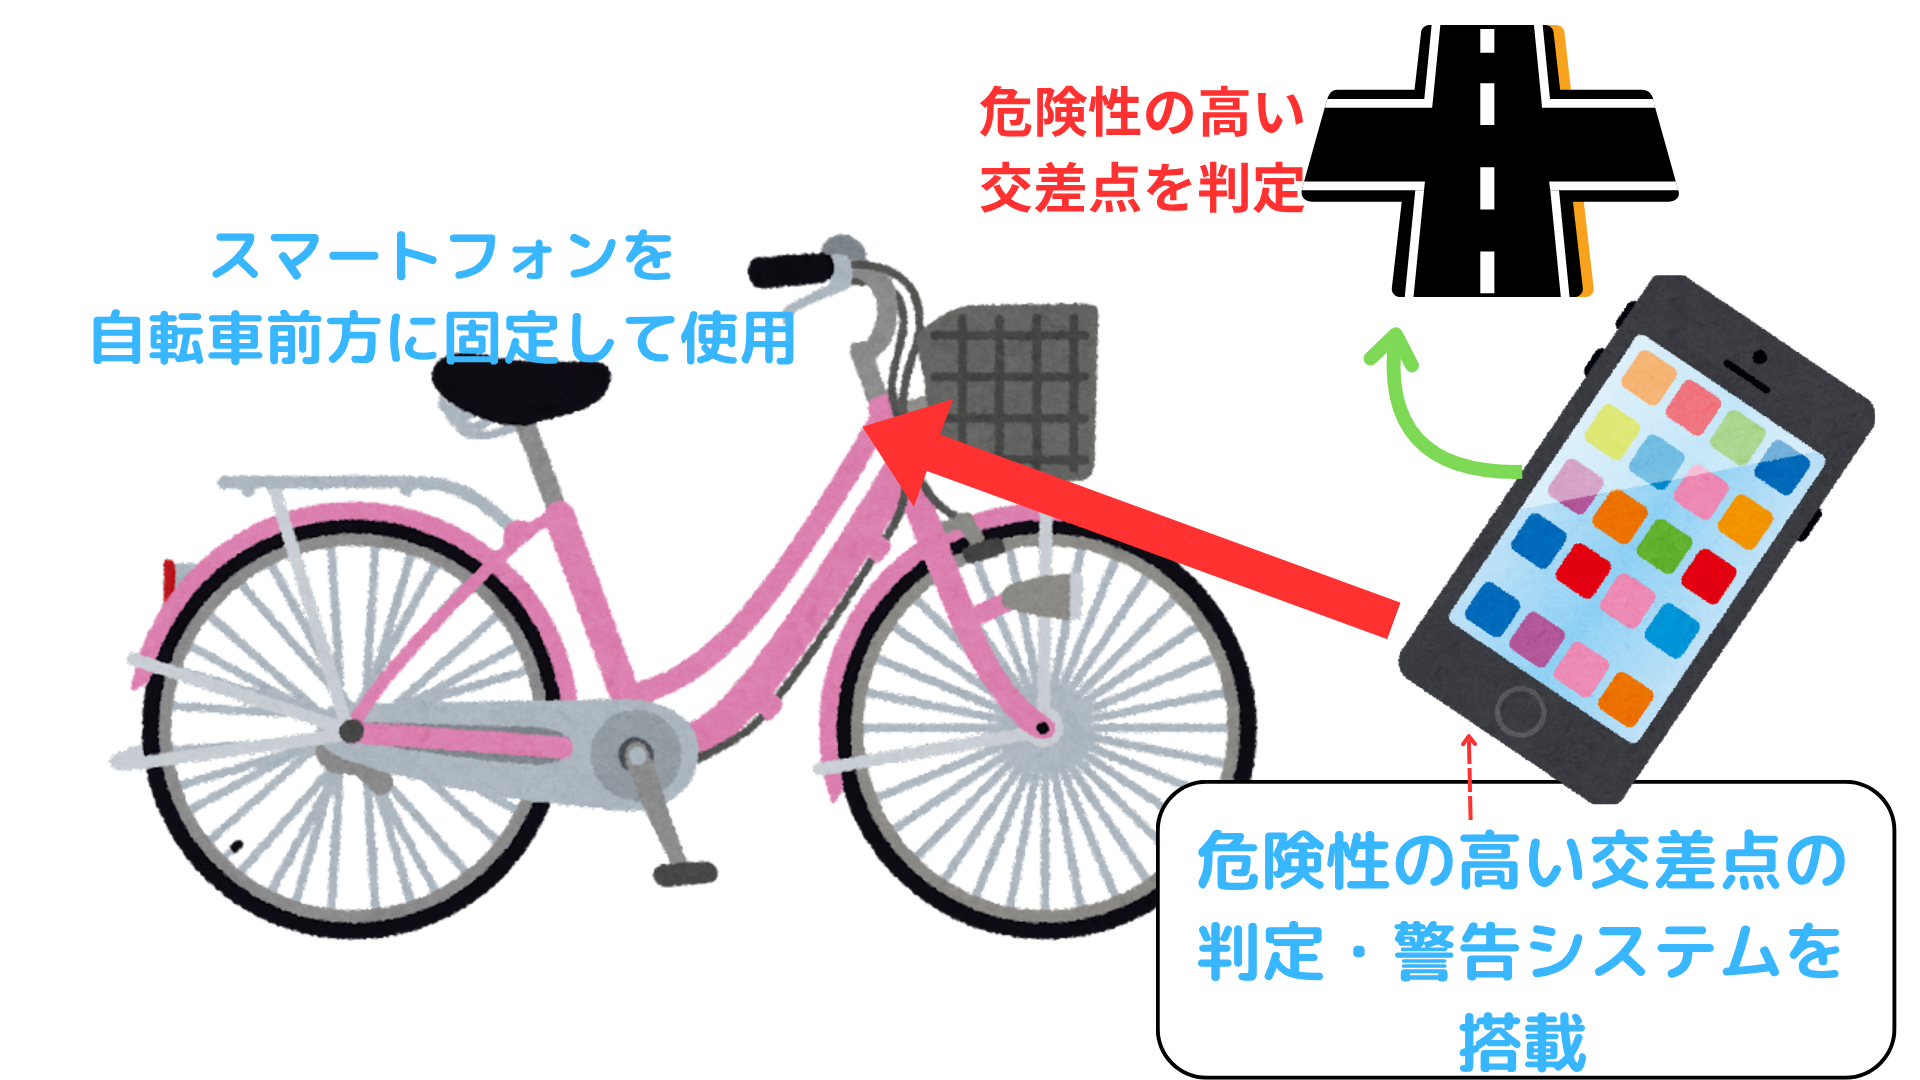
\includegraphics[width=14cm]{./Figs/gainenzu_final.png}
  \caption{危険交差点警告システムの概念図}
  \label{fig:idea}
\end{figure}

\vspace{0.75cm}

\indent
システムの構成要素を表1に,システムの概念図を図1に示す.
表1に示すように,本システムは主に4つの要素から構成される.
まず,使用者の位置情報を取得するためのGPSである.GPSを用いることで,
使用者の正確な位置情報をリアルタイムで取得することができる.
\par
次に,Google Maps Static APIを用いて使用者の周辺の交差点情報を取得する.
これは高解像度の航空画像を取得できるAPIであり,AIの画像処理に適している.
ドキュメントが豊富で導入が容易であることも採用理由の一つである.
\par
また,交差点危険度分類モデルは,機械学習により画像から危険な交差点を検出する.
道路の形状から交差点を判定し,さらに形状・塀・街路樹などの障害物から危険度を分類する.
危険度によって道路を分類することで,すべての交差点に近づくたびに作動することを防ぎ,必要な場合のみ警告を行うことができる.
\par
最後に,警告システムは危険性の高い交差点が検出された場合,音声とバイブレーションで警告を行う.
光やアラームは,騒音問題になったり明るい時間帯では気が付かない可能性があるため,本システムでは搭乗者のみに伝わる手段を採用した.

\subsection{AIの学習方法}

ここでは,システムの動作の流れを説明する前に,交差点危険度分類モデルの学習方法について説明する.
学習データとしては,様々な地域での道路の航空画像を収集し,それらの画像に対して,交差点か否か・交差点の危険度をラベル付けする.
この際,交差点の画像のみでなく,交差点ではない道路の画像も収集することで,AIモデルが交差点と非交差点を正確に識別できるようにする.
\par
また,交差点の危険度については,例えば,交差点の形状や塀や街路樹などの障害物の有無を考慮して,「非交差点」「安全な交差点」「危険な交差点」の3段階に分類する.
このようにして収集したデータを用いて,交差点危険度分類モデルを作成する.また,道路の形状においては,十字路やT字路だけでなく五差路といった複雑な形状も考慮する.
\par
本システムでは,画像認識技術として畳み込みニューラルネットワーク(Convolutional Neural Network)を採用する.
畳み込みニューラルネットワークは,画像の特徴を自動的に学習する深層学習手法であり,特に画像分類や物体検出において一般的に用いられる\cite{ref:newral}.
畳み込みニューラルネットワークは,畳み込み層,プーリング層,全結合層から構成されており,畳み込み層では画像の局所的な特徴を抽出し,
プーリング層では特徴マップのサイズを削減して計算効率を向上させる.
全結合層では,抽出された特徴を基に最終的な分類を行う.
\par
交差点危険度分類においては,畳み込みニューラルネットワークが道路の形状パターン,障害物の配置,交通環境などの複雑な視覚的特徴を学習し,
これらの特徴から交差点の危険度を自動的に判定する.
従来の画像処理手法と比較して,畳み込みニューラルネットワークは大量の学習データから自動的に特徴を抽出できるため,
より高精度で汎用性の高い交差点認識が可能となる.
\par

\subsection{システム動作フロー}

\begin{figure}[H]
  \centering
  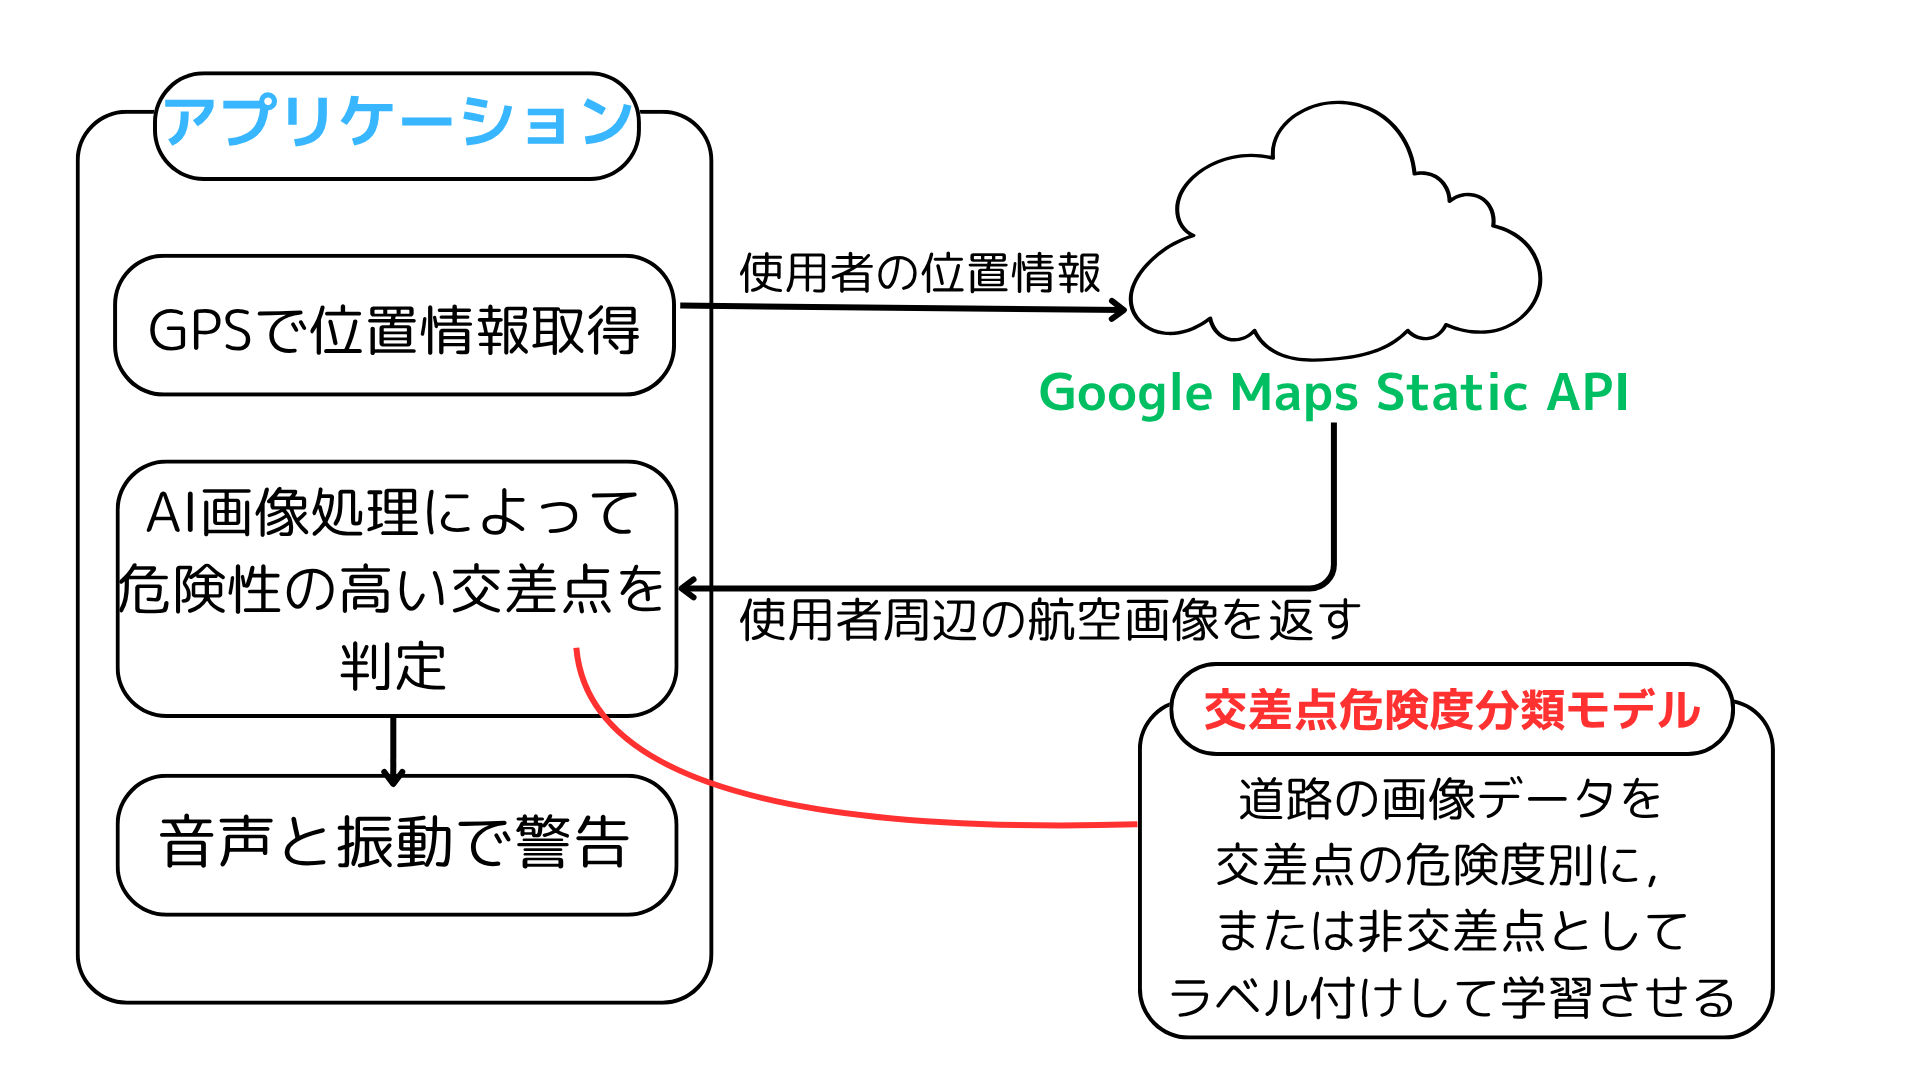
\includegraphics[width=14cm]{./Figs/system_new.png}
  \caption{危険交差点警告システムのシステム構成図.GPSから入力される位置情報を元に,Google Maps APIを用いて周辺の航空画像を取得し,AIによる画像処理を行う.
  危険性の高い交差点が検出された場合,搭乗者に音声とバイブレーションで警告を行う.アラームと違い,音声とバイブレーションは騒音を発生させないため,周囲の人に迷惑をかけることなく,搭乗者にのみ警告を行うことができる.}
  \label{fig:system}
\end{figure}

\indent
本システムの動作の流れを図\ref{fig:system}に示す.
まず,入力としては,スマートフォンのGPSから位置情報を取得する.
次に,Google Maps Static APIを用いて,現在地周辺の航空画像を取得する.
この航空画像は,使用者の現在地を中心とした一定範囲の画像である.
\par
取得した航空画像は,事前に学習させた畳み込みニューラルネットワークによって処理される.
道路の形状や障害物の配置などを解析し,交差点の有無と危険度を自動判定する.
\par
こうして危険性の高い交差点が検出された場合,搭乗者に対して音声とバイブレーションで警告される.
具体的には,スマートフォンから日本語の音声で「危険な交差点があります.注意してください」といった警告が行われるとともに,
バイブレーション機能を用いて触覚的な警告も同時に行われる.
これは,搭乗者が注意を払うべき危険な交差点が近くにあることを知らせるためのものである.
\par


\section{提案手法の実現可能性の評価と妥当性の検証}

\subsection{主張・手法のまとめ}
\indent
本提案は,自転車搭乗者の注意力の限界を補い,出会い頭衝突の事故を防ぐための危険交差点警告システムである.
具体的には,GPSを用いて使用者の位置情報を取得し,Google Maps Static APIを用いて現在地周辺の航空画像を取得する.
その後,AIによる画像認識技術を用いて交差点を検出し,搭乗者に音声とバイブレーションで警告を行う.
このシステムにより,自転車搭乗者は危険な交差点を事前に認識し,注意を払うことができるため,出会い頭衝突の事故を減少させることが期待される.
\par

%提案手法の実現可能性を評価する.
\subsection{実現可能性の評価}
\indent
ここからは,提案手法の実現可能性について評価する.
提案手法は,主にGPSとGoogle Maps Static APIを用いて現在地周辺の航空画像を取得し,AIによる画像認識技術を用いて交差点を検出する.
これらの技術は,現在の技術水準で十分に実現可能である.
特に,GPSは現在のスマートフォンに標準装備されており,位置情報の取得は容易である.
また,Google Maps Static APIは,Googleが提供するAPIであり,現在地周辺の航空画像を簡単に取得できる.
さらに,AIによる画像認識技術は,近年の深層学習の進展により,精度が向上しており,交差点の検出も十分に可能である.
\par
まず,Google Maps Static APIによる航空画像の取得の範囲について定量的に評価する.
Google Maps Static APIは,zoomレベルを指定することで,航空画像の拡大率を調整できる.これにより,現在地周辺の航空画像を取得する際の範囲を調整できる.
本システムでは,zoomレベルを19に設定する.zoomレベルが19の場合,1ピクセルあたりの地上距離は$0.2986m$であり,
画像の取得範囲は,(1)のようになる\cite{ref:zoomrevel}.

\begin{align}
\mathrm{取得範囲} = \frac{S\times m/px}{2} = \frac{640 \times 0.2986}{2} = \frac{191.104}{2} ≈ 95.55 \text{ m}
\end{align}
($m/px$: 1ピクセルあたりの地上距離, $S$:画像サイズ )
\vspace{0.75cm}

よって,Google Maps Static APIを用いて取得できる航空画像の範囲は,現在地を中心に約95.55m四方となる.
この範囲は,通常の自転車の走行速度約15km/hであれば,約14秒間隔で取得できるため,十分な頻度で航空画像を取得できる.
\par

\indent
次に,AIによる画像認識技術の精度について評価する.
提案手法では,航空画像に対してAIを用いて交差点の有無およびその危険性を判定するため,AIモデルの識別精度が重要である.
この評価には,あらかじめ「非交差点」「安全な交差点」「危険な交差点」の3クラスで人手でラベル付けされた航空画像データセットを用い,AIによる分類結果との一致度を確認する.
また,評価指標としては,表\ref{tab:evaluation_metrics}のような5指標を用いる.

\begin{table}[H]
  \centering
  \caption{提案手法の評価指標(三段階分類:非交差点・安全な交差点・危険な交差点)}
  \label{tab:evaluation_metrics}
  \begin{tabular}{|c|c|}
    \hline
    指標 & 説明 \\ \hline
    Precision(各クラス) & 各クラスで正しく判定した割合 \\ \hline
    Recall(各クラス) & 各クラスの実際のデータを正しく判定した割合 \\ \hline
    F1スコア(各クラス) & PrecisionとRecallの調和平均(各クラス) \\ \hline
    Macro平均 & 各クラスの指標の平均値 \\ \hline
    Accuracy & 全体の正解率 \\ \hline
  \end{tabular}
\end{table}

ここからは,「非交差点」「安全な交差点」「危険な交差点」の三段階で評価する多クラス分類問題として,Precision,Recall,F1スコアを各クラスごとに算出し,その平均(Macro平均)とAccuracyを用いて認識性能を評価する.
これらの指標は,画像分類や物体検出における多クラス評価で標準的に用いられている \cite{powers2011evaluation, padilla2021comparative}.
特にMacro平均とF1スコアは,クラス間のバランスを考慮した指標として有用である \cite{saito2015precision}.
各指標は(2)〜(6)の数式で表される.

\begin{align}
\mathrm{Accuracy} &= \frac{\sum_{i=1}^{N} TP_i}{\sum_{i=1}^{N} (TP_i + FP_i + FN_i)} \\
\mathrm{Precision}_i &= \frac{TP_i}{TP_i + FP_i} \\
\mathrm{Recall}_i &= \frac{TP_i}{TP_i + FN_i} \\
\mathrm{F1}_i &= 2 \cdot \frac{\mathrm{Precision}_i \cdot \mathrm{Recall}_i}{\mathrm{Precision}_i + \mathrm{Recall}_i} \\
\mathrm{Macro\text{-}F1} &= \frac{1}{N} \sum_{i=1}^{N} \mathrm{F1}_i
\end{align}

\vspace{1cm}

ここで,$i$は「非交差点」「安全な交差点」「危険な交差点」の各クラスを表し,$TP_i$はクラス$i$を正しく判定した件数,$FP_i$は他クラスを誤ってクラス$i$と判定した件数,$FN_i$はクラス$i$を他クラスと誤判定した件数である.
これらの指標を用いることで,三段階の危険度分類における提案手法の認識性能を定量的に評価できる.
\par
今回は,実際のデータが存在しないため,各指標の目標値を設定し,それをもとに本提案の実現可能性を評価する.
従来のアルゴリズムベースの手法は,事前定義されたルールに基づくため,
複雑な形状や多様な障害物など非定型的な状況への対応に限界がある\cite{technolynx_dl_vs_traditional, mdpi_comprehensive_survey_dl_image_processing, peerj_intersection_prediction}.
一方,本システムでは各評価指標の目標値を以下のように設定する:
Precision,Recall,F1スコア,Macro平均をそれぞれ0.8以上,Accuracyを0.85以上とする.
先行研究によれば,AIを用いた道路のセマンティックセグメンテーション技術は,走行可能領域の識別において約80\%から90\%の精度を達成している
\cite{ref:road_segmentation}.そのため,提案手法においても同等の精度を目指すことは現実的であると考えられる.
\par
既存の交通安全システムや警告技術は様々な形で導入されており,例えば,一般的なテレマティクスシステムを導入した企業では,
事故件数が導入前と比較して30\%減少した事例も報告されている\cite{ref:telematics}.また,交差点に設置される衝突警告システム (ICWS: Intersection Conflict Warning Systems) は,
特定の条件下において事故を3.5\%から19\%以上減少させる効果が示されている\cite{ref:fhwa}。
しかし,これらの既存システムは自動車向けであったり,固定インフラに依存したりすることや,過去のデータに基づく警告に留まることが多い.
そのため,自転車という移動手段の特性や,視界の悪い場所や複雑な形状の交差点といった非定型的な状況における事故防止に対しては,十分な対応が難しい場合がある.
本システムのAIは、交差点の危険度判定においてAccuracy 85\%以上、Precision、Recall、F1-scoreのMacro平均で0.8以上という高い認識精度を目標としている。
この高精度なAIによるリアルタイムの危険度判定と警告により,既存のシステムでは危険性の判断が難しい「道路の複雑な形状や視界の悪さ」に対しても対応でき,
本システムの認識精度が目標値を達成できれば,現状の事故率52.9\%から,目標とする約10\%の削減に貢献できると考えられる.
\par
\begin{table}[H]
  \centering
  \caption{本システムの消費電力}
  \label{tab:power_consumption}
  \begin{tabular}{|c|c|c|}
    \hline
    構成要素 & 消費電力 (W) & 備考 \\ \hline
    GPS & 0.05 & 常時使用 \\ \hline
    Google Maps Static API & 0.02 & リクエストごとに消費 \\ \hline
    AIによる画像認識 & 0.1 & 一回の処理で消費 \\ \hline
    警告システム & 0.03 & 音声とバイブレーションで消費 \\ \hline
    合計 & 0.2 & 一回の処理あたりの合計消費電力 \\ \hline
\end{tabular}
\end{table}
消費電力についても評価する.本システムの消費電力を表\ref{tab:power_consumption}に示す.
GPSは常時使用するため,0.05Wの消費電力が必要である.
Google Maps Static APIは,リクエストごとに0.02Wの消費電力が必要である.
AIによる画像認識は,一回の処理で0.1Wの消費電力が必要である.
警告システムは,音声とバイブレーションで0.03Wの消費電力が必要である.
これらを合計すると,一回の処理あたりの消費電力は0.2Wとなる.
\par
AppleのiPhone 15を例にとると,iPhone 15のバッテリー容量は約3279mAhであり,電圧は3.85Vであるため,バッテリーのエネルギー量は約12.6Whとなる\cite{iphone_battery}.
この場合,提案手法の消費電力は0.2Wであるため,バッテリーのエネルギー量から考えると,理論上は約63時間の連続使用が可能である.
実際には,熱などによりバッテリーの効率が低下するため,連続使用時間はさらに短くなると予想されるが,
GPSやAIによる画像認識の処理は,常に行われるわけではなく,使用者が自転車に乗っている間のみ行われるため,
実際の使用においては,提案手法はスマートフォンのバッテリーで十分に動作可能であると考えられる.
\par

\subsection{妥当性の検証}
\indent
次に,提案手法の妥当性についてを説明する.
本システムの危険交差点の判別においては,危険の定義を「見通しの悪さ」とし,具体的には交差点の形状や周囲の障害物の有無などを考慮した.
この場合,AIではなくアルゴリズムを用いることのほうが妥当であるとも考えられるが,
AIを用いることで,より柔軟に危険な交差点を検出できると考える.アルゴリズムでは,事前に定義されたルールに基づいて危険な交差点を検出するため,特定の条件に合致しない場合は検出できない可能性がある.
一方で,AIを用いることで,事前に定義されたルールに依存せず,画像の特徴を学習し,危険な交差点を検出することができる.
例えば,交差点の形状が複雑であったり,周囲の障害物が多かったりする場合でも,AIはその特徴を学習し,危険な交差点を検出することができる.
\par
また,モジュールとして実装してしまうと,天候や時間帯によって認識精度が変化することや,高いコストがかかる
という懸念点があるが,
本システムはアプリケーションとして導入するため,GPSによるリアルタイムでの位置情報取得が行えるのに加え,
Google Maps Static APIを用いて周辺の航空画像を取得するため,常に晴天時の昼間の画像を取得することができ,
認識精度の変化を抑えることができる.また,アプリケーション実装により,専用ハードウェアと比較して大幅なコスト削減が可能である.
モジュール実装では部品費用,防水・防塵対策,量産体制構築等により1台あたり数万円から数十万円のコストが発生するが,
本システムでは既存のスマートフォンを活用するため,ユーザーの追加費用負担や開発者の製造・配送コストが不要である.
\par
さらに本提案では交差点の判定の際,過去の事故データではなく,航空画像を用いた.
過去の事故データに基づく手法では,特定の地域や環境においては有効であるが,地域によっては事故データが少ない場合や,
事故の発生頻度が低い場合には,十分な精度で危険な交差点を検出できない可能性がある.
そのため,過去の事故データに依存せず,航空画像を用いて危険な交差点を検出することは,地域や環境に関係なく,より広範囲での適用が可能である.
\par
また,本提案は自転車搭乗者の行動変容を促すことを目的としているため,法令違反や不注意を完全に無くすことは難しいが,
自転車搭乗者に対して自動かつ適切な注意喚起を行うことで,事故のリスクを低減できると考える.
特に,交差点などの危険な場所での注意喚起は,自転車搭乗者の注意力の限界を補い,事故を防ぐことができるため,自転車事故の怪我人や死者数を減少させることが期待される.
これにより,アルゴリズムでは対応しきれない複雑な環境においても,安定して高い検出性能を発揮できると考えられる.この高精度なAI検出により、
自転車での出会い頭衝突事故率を現状から約10\%減少させることは,段階的に積み重ねることで,最終的には達成できると考えられ,
本提案は自転車事故率の低減に関して妥当であると考える.
\par


\section{おわりに}
\indent
本提案では,自転車搭乗者の注意力の限界を補い,出会い頭衝突の事故を防ぐための危険交差点警告システムを提案した.
具体的には,GPSを用いて使用者の位置情報を取得し,Google Maps Static APIを用いて現在地周辺の航空画像を取得する.
その後,AIによる画像認識技術を用いて,危険性の高い交差点を検出し,搭乗者に音声とバイブレーションで警告を行う.
このシステムにより,自転車搭乗者は危険な交差点を事前に認識し,注意を払うことができるため,出会い頭衝突の事故を減少させることが期待される.
\par
今後の課題としては,提案手法の実装と評価を行い,実際の使用環境においても高い精度で危険な交差点を検出できるようにすることが挙げられる.
また,交差点危険度分類モデルには膨大な学習データが必要であり,特に多様な地域や環境におけるデータを収集することが重要である.
さらに,提案手法の認識精度を向上させるために,AIモデルの再学習やパラメータ調整を定期的に行うことも必要である.
\par
最後に,本提案の実現に向けては,技術的な課題や社会的な課題もあるが,これらを克服することで,自転車搭乗者の安全な移動を支援し,
出会い頭衝突の事故を減らすことができると考える.学習させるデータを多く集めることで認識精度を向上させることも可能である.
認識精度が高まることで危険を可視化でき,使用者の交通安全意識を向上させることができるため,本提案の目的である自転車での出会い頭衝突の事故率を約10\%減少させることが可能になると考える.
今後の展望としては,自転車以外の交通手段にも応用することで,より広範な交通安全の向上を目指す.
\par


\begin{thebibliography}{9}
\bibitem{ref:koutuusyou_1} 国土交通省, 「自転車活用推進計画」, \url{https://www.mlit.go.jp/road/bicycleuse/good-cycle-japan/assets/pdf/jitensha_katsuyo.pdf}.
\bibitem{ref:koutuusyou_2}  国土交通省, 「第1回自転車の活用推進に向けた有識者会議 自転車の活用に関する現状について」, \url{https://www.mlit.go.jp/road/ir/ir-council/bicycle-up/06pdf/02.pdf}.
\bibitem{ref:sonpo_1} 一般社団法人 日本損害保険協会, 「自転車の事故 〜安全な乗り方と事故への備え〜2024年8月版」, \url{https://www.sonpo.or.jp/report/publish/koutsu/g34l0i0000006z5o-att/book_bicycle.pdf}.
\bibitem{ref:keisatu_1} 警察庁, 日本損害保険協会, 「自転車関連交通事故の状況」, \url{https://www.npa.go.jp/koutsuu/kikaku/bicycle/kentokai/01/siryou07.pdf}.
\bibitem{ref:newral} 内田祐介 山下隆義,「物体認識のための畳み込みニューラルネットワークの研究動向」,\url{https://search.ieice.org/bin/pdf_link.php?category=D&lang=J&year=2019&fname=j102-d_3_203&abst=}
\bibitem{powers2011evaluation} 
D. M. W. Powers, 「Evaluation: From Precision, Recall and F-measure to ROC, Informedness, Markedness and Correlation,」, 2011.
\bibitem{padilla2021comparative}
R. Padilla, W. L. Netto, and E. A. da Silva, 「A Comparative Analysis of Object Detection Metrics with a Companion Open‐Source Toolkit,」, 2021.
\bibitem{ref:zoomrevel}
Microsoft,「Zoom levels and tile grid」,\url{https://learn.microsoft.com/en-us/azure/azure-maps/zoom-levels-and-tile-grid?tabs=csharp}
\bibitem{saito2015precision}
T. Saito and M. Rehmsmeier, 「The Precision-Recall Plot Is More Informative than the ROC Plot When Evaluating Binary Classifiers on Imbalanced Datasets,」, 2015.
\bibitem{technolynx_dl_vs_traditional} TechnoLynx, 「Deep Learning vs. Traditional Computer Vision Methods」, \url{https://www.technolynx.com/post/deep-learning-vs-traditional-computer-vision-methods}.
\bibitem{mdpi_comprehensive_survey_dl_image_processing} MDPI, 「A Comprehensive Survey of Deep Learning Approaches in Image Processing」, \url{https://www.mdpi.com/1424-8220/25/2/531}.
\bibitem{peerj_intersection_prediction} PeerJ, 「Intersection collision prediction and prevention based on vehicle-to-vehicle (V2V) and cloud computing communication」, \url{https://peerj.com/articles/cs-2846.pdf}.
\bibitem{ref:road_segmentation}
Zhaoxiang Wang, Kaiqi Huang, 「Road Scene Semantic Segmentation Based on Deep Learning」, 2023.
\bibitem{ref:telematics} 日本カーソリューションズ, 「自動車事故ゼロも夢じゃない「テレマティクスサービス」とは?」, 
\url{https://www.ncsol.co.jp/telematics/column/001.html}
\bibitem{ref:fhwa} Federal Highway Administration, 「Intersection Conflict Warning System Human Factors: Final Report」, 
\url{https://www.fhwa.dot.gov/publications/research/safety/16061/16061.pdf}
\bibitem{iphone_battery}
Apple, 「iPhone | Apple公式サイト」, \url{https://www.apple.com/jp/iphone-15/specs/}.


\end{thebibliography}

\end{document}